\task{Модельки}
\begin{itemize}
\itA Свойства подобных фигур говорят нам, что объём фигур, подобных с коэффициентом $k$, различается в $k^3$ раз. Масса тела равна плотности вещества, умноженной на взятый его объём — поэтому она также должна уменьшаться в $k^3$ раз при уменьшении тела в $k$ раз.

В свою очередь, $1200\,/\,43^3 = 0.015$: 15 граммов — слишком маленький вес для модельки, но это вполне объяснимо: сделана она всё-таки грубее, чем оригинальная машина, и металл в ней сравнительно более толстый.

\itB Мы хотели бы отметить, что длина меридиана, \SI{40000}{\text{километров}}, это {\bf вся окружность} Земли, а не её половина. То есть Парижский меридиан проходит через две долготы: \SI{2.33^\circ}{\text{в.\,д.}} и \SI{177.67^\circ}{\text{з.\,д.}}.

Таким образом, самолёту нужно пролететь \SI{40000}{\text{км}}, затрачивая на километр $0.54$ минуты. $40000 \cdot 0.54 \div 60 = \SI{360}{(\text{часов})}$.

\itC С одной стороны, если есть «классическая» плоская система из шестерёнок, то в ней передача вращения симметрична. С другой — можно с применением некоторой креативности придумать «несимметричную» систему. Например, такую, как на рисунке:

\begin{center}
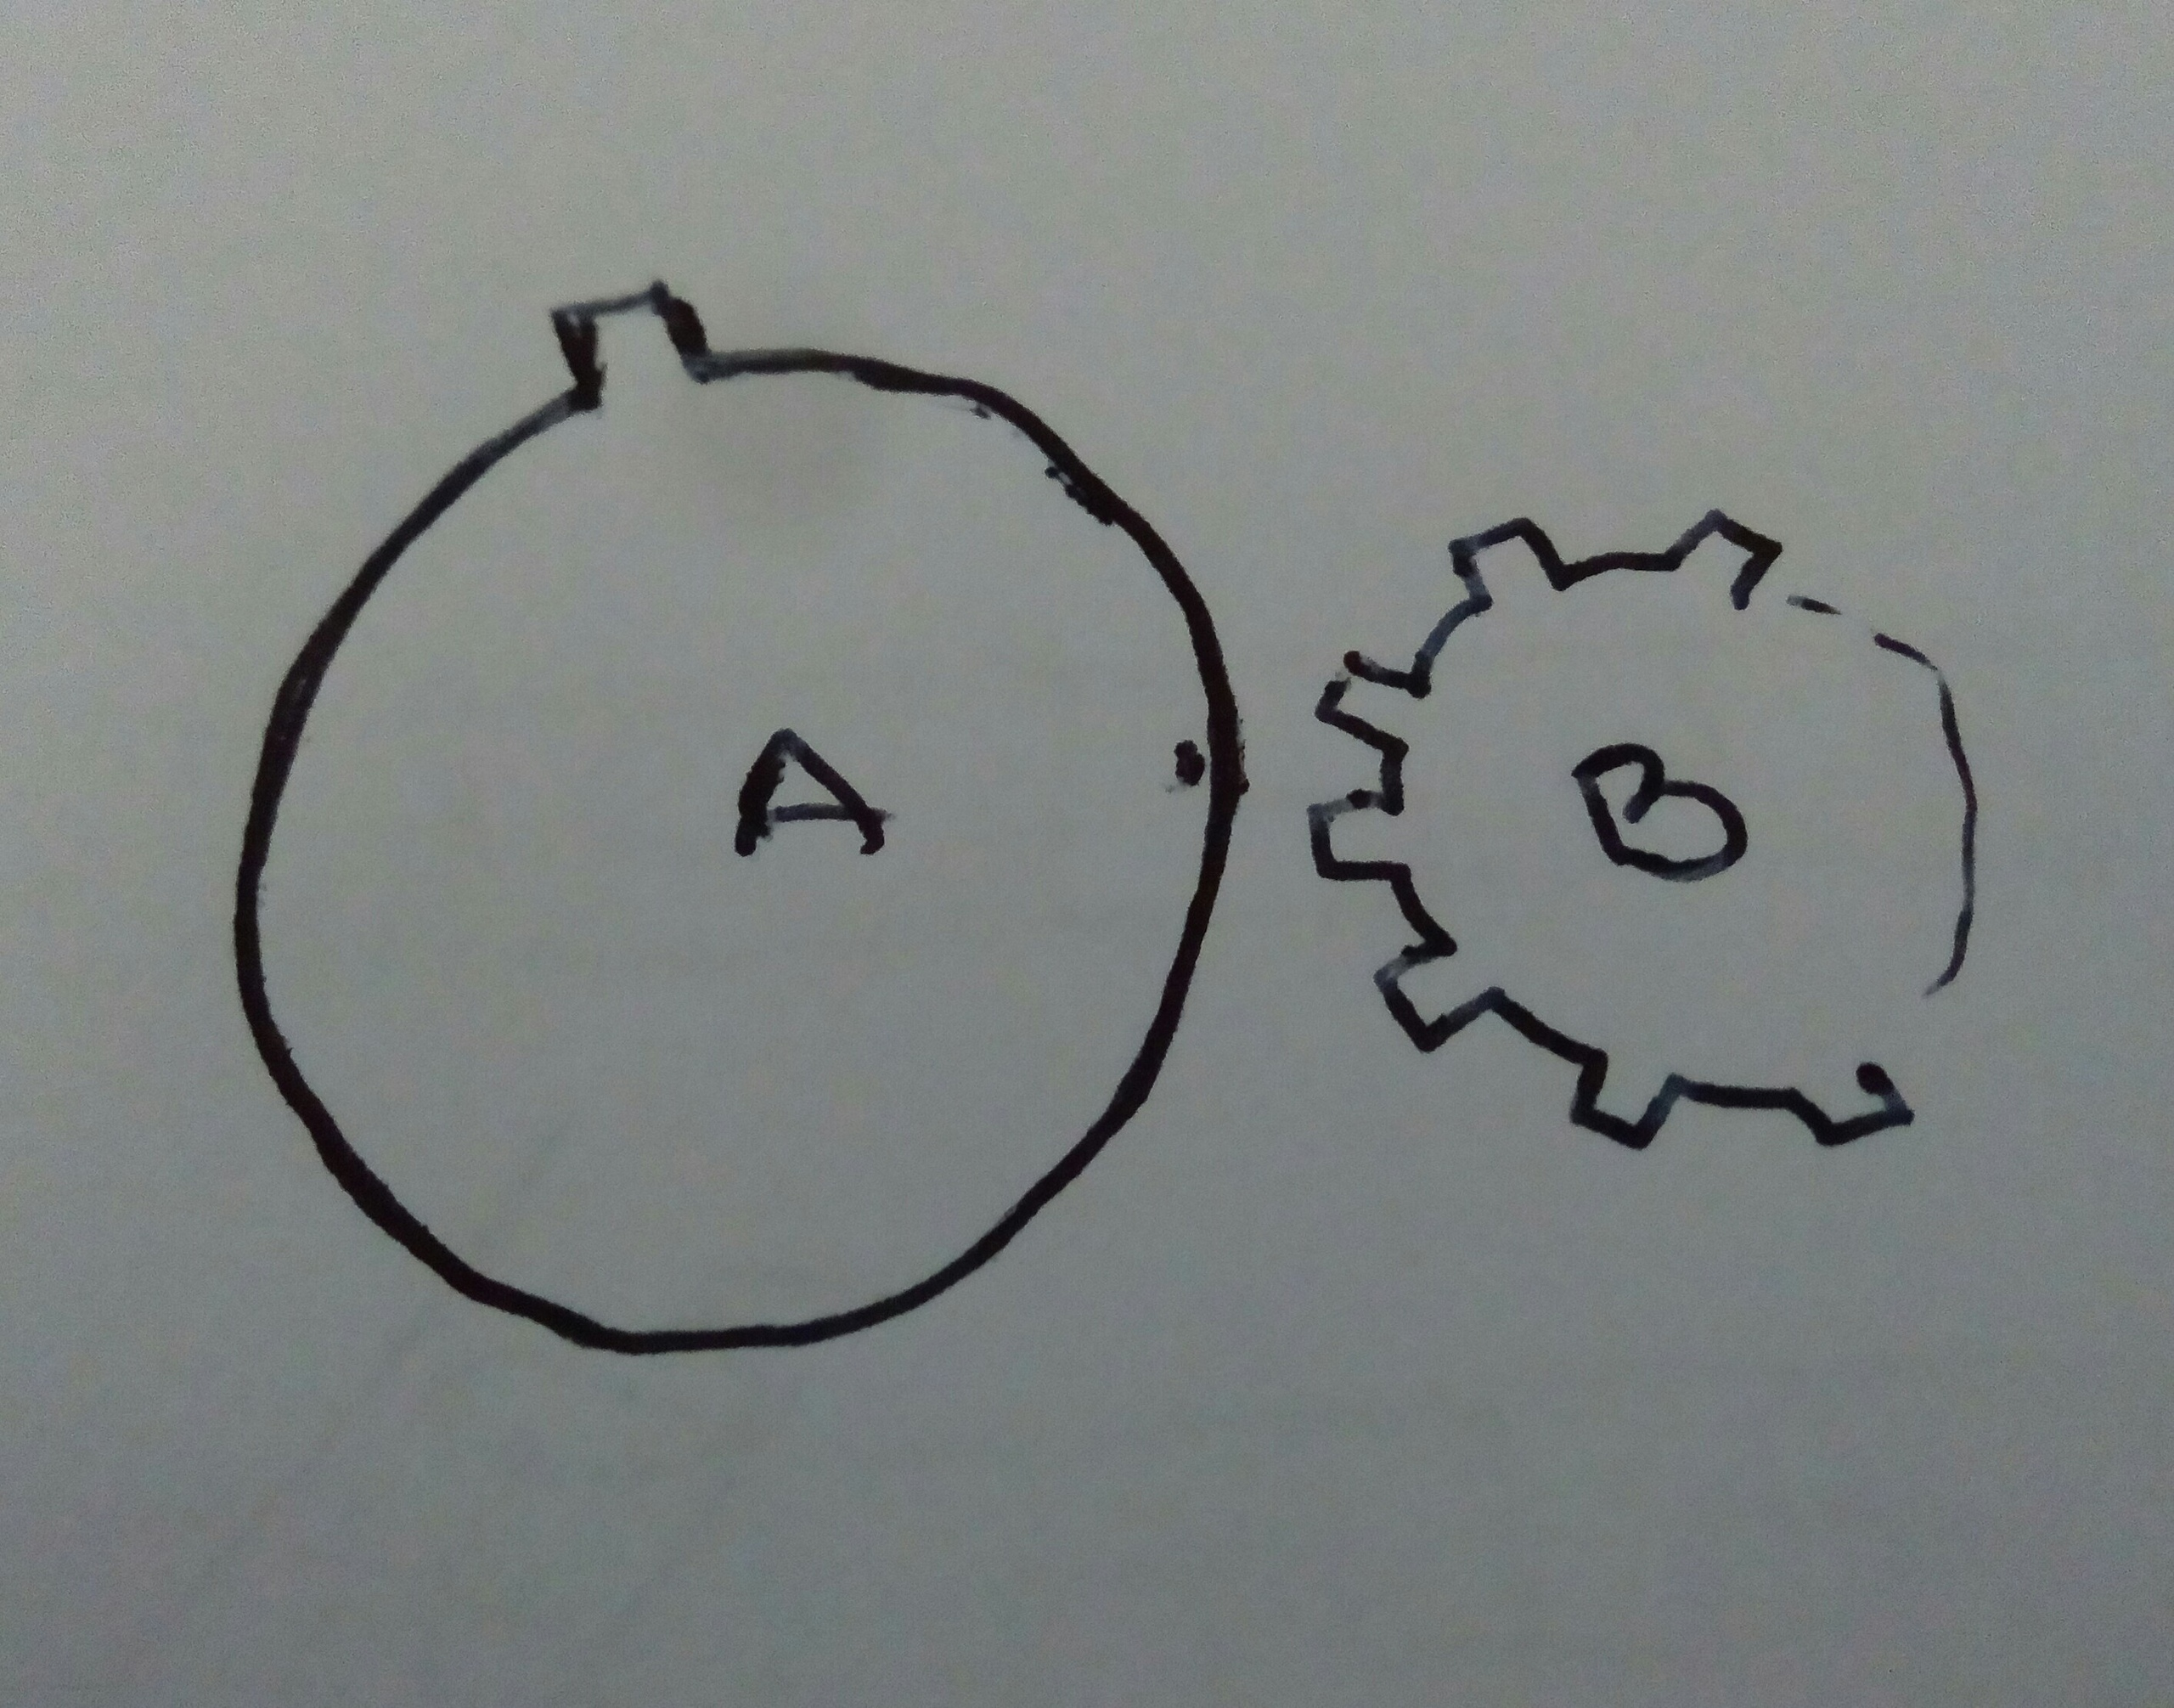
\includegraphics[natwidth=2560,natheight=2011,width=6cm]{figures/2018-models}
\end{center}

При вращении шестерёнки $A$ она каждый оборот будет цепляться своим единственным зубом за шестерёнку $B$, и та будет вращаться. При вращении же шестерёнки $B$ в текущем положении шестерёнок она не будет касаться $A$ и передавать ей вращение.

\end{itemize}